%auto-ignore
\documentclass[tikz]{standalone}

\usetikzlibrary{calc}

\begin{document}
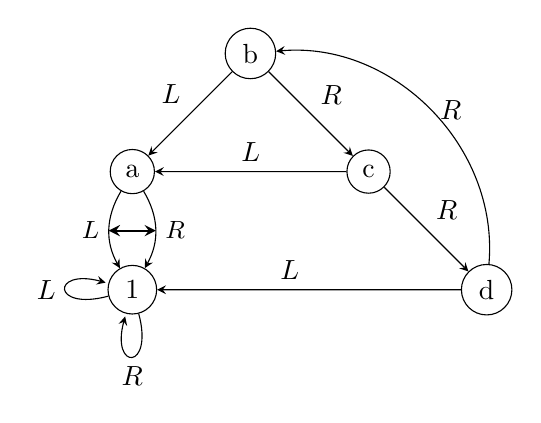
\begin{tikzpicture}[scale=1.5,>=stealth]

\node [circle,draw=black] (n0) at ( 0,  0) {b};
\node [circle,draw=black] (n1) at ( 1, -1) {c};
\node [circle,draw=black] (n2) at ( 2, -2) {d};

\node [circle,draw=black] (m1) at (-1, -1) {a};
\node [circle,draw=black] (m3) at (-1, -2) {1};

\path[->]
	(m3) edge [loop below] node [below] {$R$} ()
	(m3) edge [loop left] node [left] {$L$} ()
;
%
%\node [circle,draw=black] (m11) at (-1-0.5, -1-0.5) {1};
%\node [circle,draw=black] (m12) at (-1+0.5, -1-0.5) {1};
\draw [<->,thick] (-1.2,-1.5) to (-0.8,-1.5);
\draw [->] (m1) to[bend left] node [right] {\small$R$} (m3);
\draw [->] (m1) to[bend right] node [left] {\small$L$} (m3);


\path[->]
	(n0) edge node [above right] {$R$} (n1)
	edge node [above left] {$L$} (m1)
	(n1) edge node [above right] {$R$} (n2)
	edge node [above] {$L$} (m1)
	(n2)
		edge node [above left] {$L$} (m3)
		edge [bend right=50] node [right] {$R$} (n0)
;

\end{tikzpicture}
\end{document}